\section{Figures}\label{sec:Elements_figures}
%\begin{figure}[ht]
%\centering
%\includesvg[scale=0.5]{svgimage}
%\caption{A svg image example}
%\label{fig:x cubedvv graph}
%\end{figure}
\begin{lstlisting}
\begin{figure}[h]
\centering
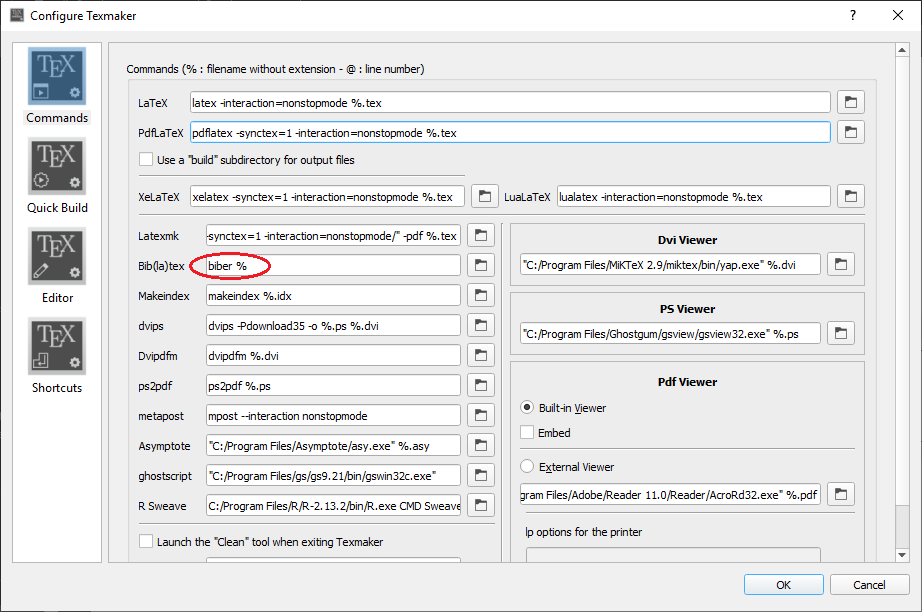
\includegraphics[width=.45\textwidth]{Intro_TexMakerConf.png}
\caption[Resume line]{An example graph}
\label{fig:example}
\end{figure}
\end{lstlisting}

\begin{figure}[h]
\centering
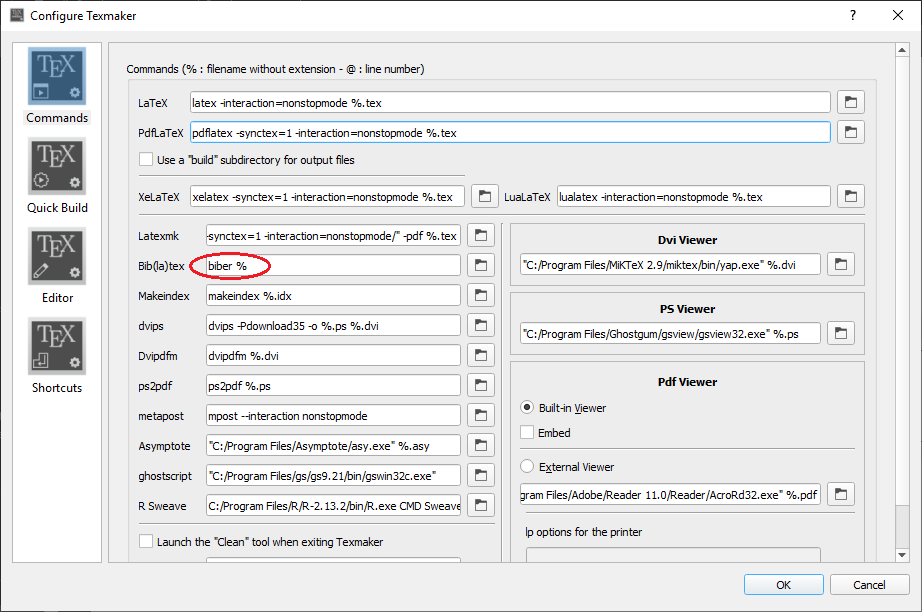
\includegraphics[width=.45\textwidth]{Intro_TexMakerConf.png}
\caption[Resume line]{An example graph}
\label{fig:example}
\end{figure}

\begin{lstlisting}
\begin{figure}[h]
    \centering
    \begin{subfigure}[b]{.3\textwidth}
        \centering
        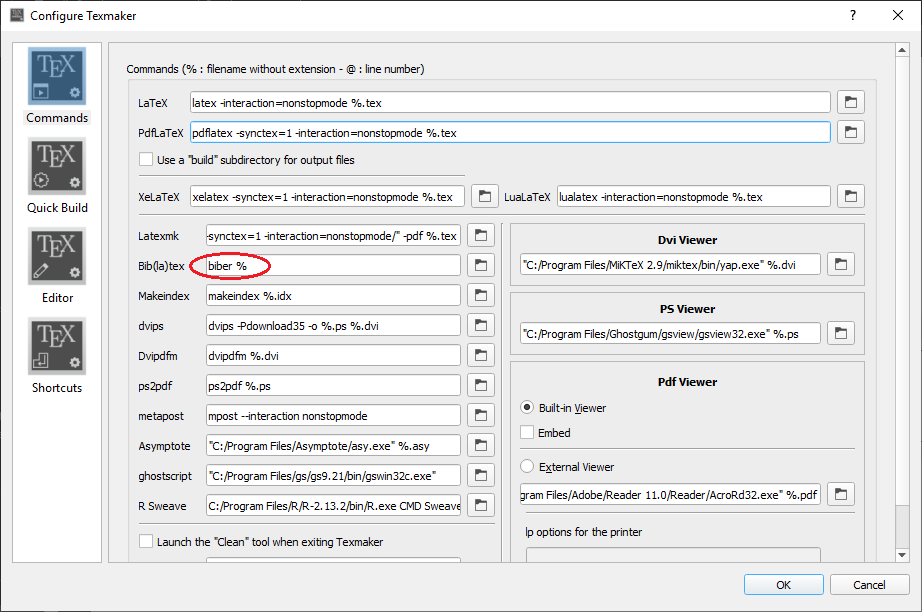
\includegraphics[width=\textwidth]{Intro_TexMakerConf.png}
        \caption{$y=x$}
        \label{fig:triple_x}
    \end{subfigure}
    \hfill
    \begin{subfigure}[b]{0.3\textwidth}
        \centering
        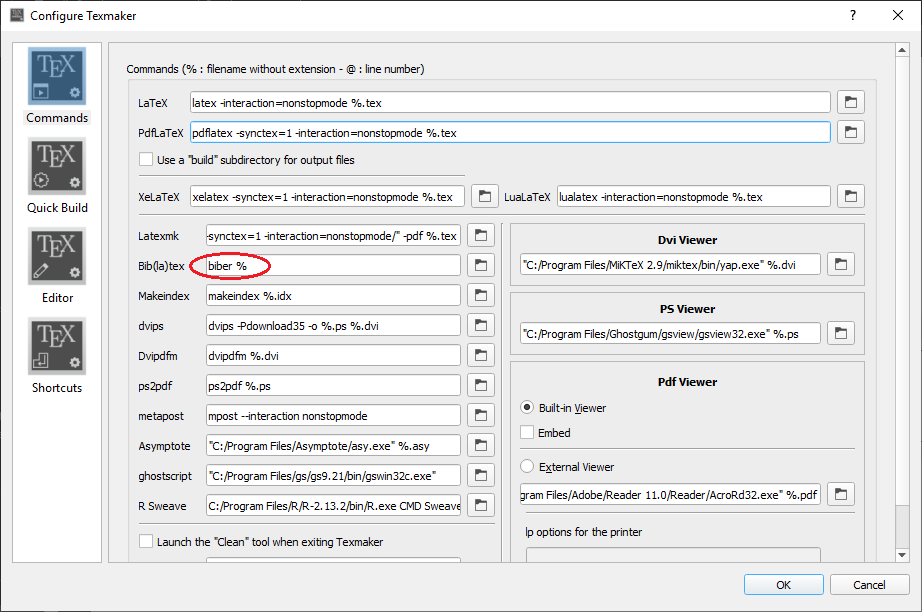
\includegraphics[width=\textwidth]{Intro_TexMakerConf.png}
        \caption{$y=3sinx$}
        \label{fig:triple_3sinx}
    \end{subfigure}
    \hfill
    \begin{subfigure}[b]{0.3\textwidth}
        \centering
        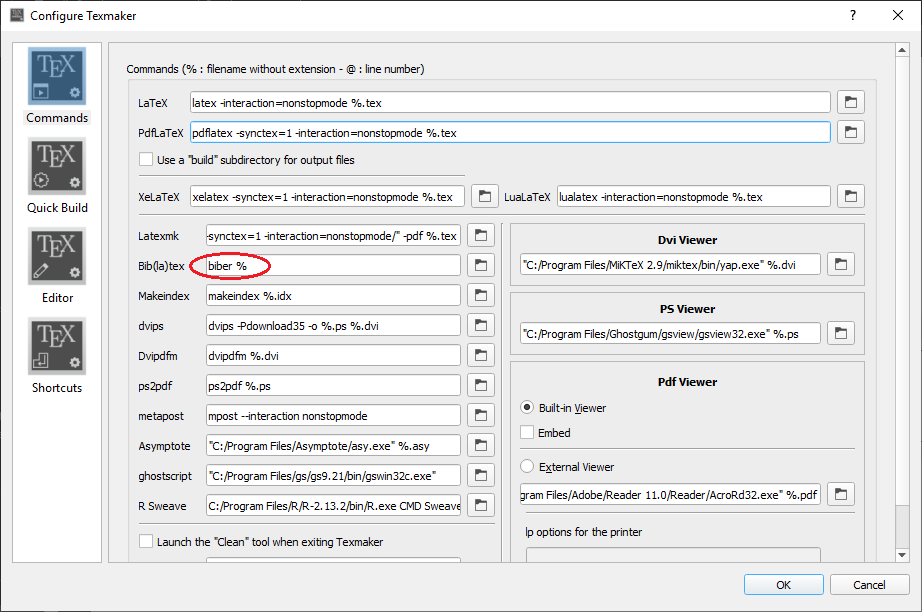
\includegraphics[width=\textwidth]{Intro_TexMakerConf.png}
        \caption{$y=5/x$}
        \label{fig:triple_5overx}
    \end{subfigure}
    \caption[Resume line]{Three simple graphs}
    \label{fig:triple}
\end{figure}
\end{lstlisting}

\begin{figure}[h]
    \centering
    \begin{subfigure}[b]{.3\textwidth}
        \centering
        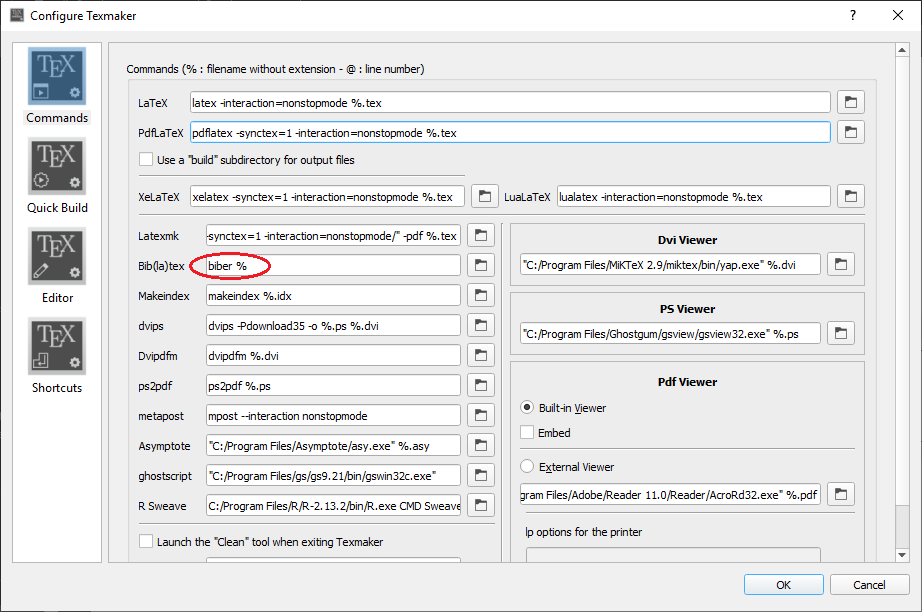
\includegraphics[width=\textwidth]{Intro_TexMakerConf.png}
        \caption{$y=x$}
        \label{fig:triple_x}
    \end{subfigure}
    \hfill
    \begin{subfigure}[b]{0.3\textwidth}
        \centering
        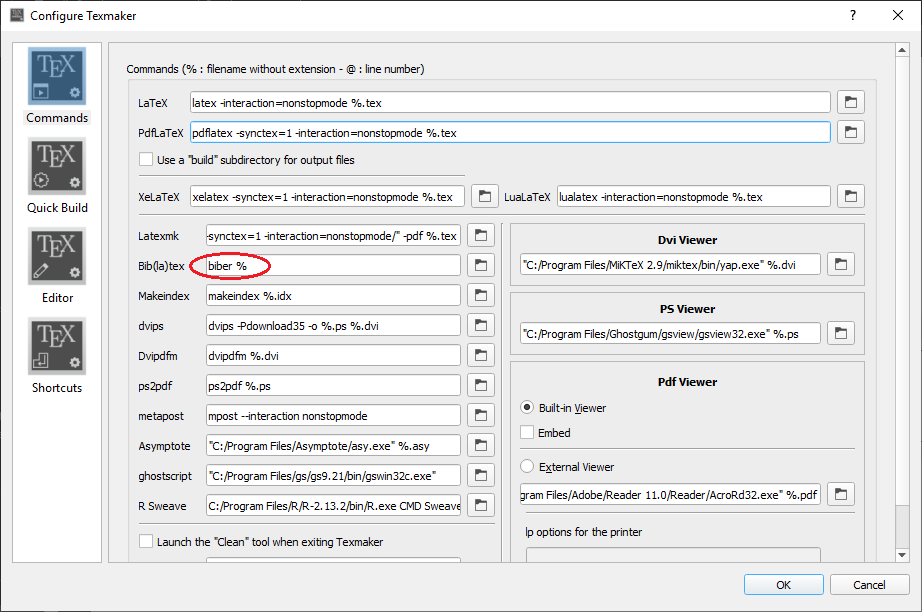
\includegraphics[width=\textwidth]{Intro_TexMakerConf.png}
        \caption{$y=3sinx$}
        \label{fig:triple_3sinx}
    \end{subfigure}
    \hfill
    \begin{subfigure}[b]{0.3\textwidth}
        \centering
        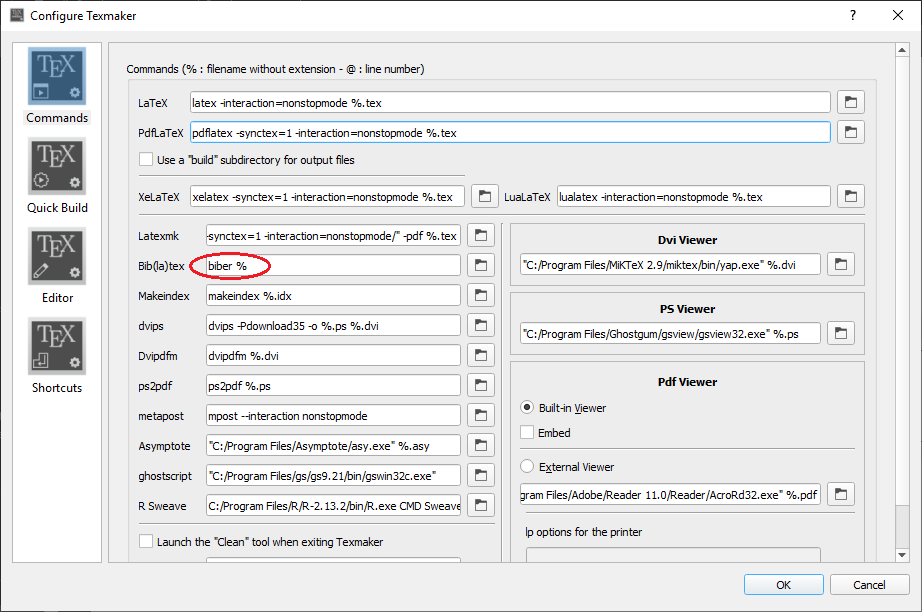
\includegraphics[width=\textwidth]{Intro_TexMakerConf.png}
        \caption{$y=5/x$}
        \label{fig:triple_5overx}
    \end{subfigure}
    \caption[Resume line]{Three simple graphs}
    \label{fig:triple}
\end{figure}